\documentclass[a4paper,conference]{IEEEtran}
\IEEEoverridecommandlockouts
\usepackage{cite}
\usepackage{amsmath,amssymb,amsfonts}
\usepackage{algorithmic}
\usepackage{graphicx}
\usepackage{textcomp}
\usepackage{xcolor}
\def\BibTeX{{\rm B\kern-.05em{\sc i\kern-.025em b}\kern-.08em
    T\kern-.1667em\lower.7ex\hbox{E}\kern-.125emX}}
\usepackage{listings}
\usepackage{alphabeta}

\begin{document}

\title{Some Capabilities of Android OS for\\ Distributed Computing\\
\thanks{978-1-6654-1042-7/21/\$31.00 ©2021 IEEE}}

\author{\IEEEauthorblockN{Gergana Mateeva}
\IEEEauthorblockA{\textit{Institute of Information and Communication Technologies} \\
\textit{Bulgarian Academy of Sciences}\\
Sofia, Bulgaria \\
gergana.mateeva@iict.bas.bg}
\and
\IEEEauthorblockN{Petar Tomov}
\IEEEauthorblockA{\textit{Institute of Information and Communication Technologies} \\
\textit{Bulgarian Academy of Sciences}\\
Sofia, Bulgaria \\
petar.tomov@iict.bas.bg}
\and
\IEEEauthorblockN{Dimitar Parvanov}
\IEEEauthorblockA{\textit{Institute of Information and Communication Technologies} \\
\textit{Bulgarian Academy of Sciences}\\
Sofia, Bulgaria \\
dimitar.parvanov@iict.bas.bg}
\and
\IEEEauthorblockN{Plamen Petrov}
\IEEEauthorblockA{\textit{Institute of Information and Communication Technologies} \\
\textit{Bulgarian Academy of Sciences}\\
Sofia, Bulgaria \\
plamen.petrov@iict.bas.bg}
\and
\IEEEauthorblockN{Georgi Kostadinov}
\IEEEauthorblockA{\textit{Institute of Information and Communication Technologies} \\
\textit{Bulgarian Academy of Sciences}\\
Sofia, Bulgaria \\
georgi.kostadinov@iict.bas.bg}
\and
\IEEEauthorblockN{Todor Balabanov\textsuperscript{\tiny{0000-0003-3139-069X}}}
\IEEEauthorblockA{\textit{Institute of Information and Communication Technologies} \\
\textit{Bulgarian Academy of Sciences}\\
Sofia, Bulgaria \\
todor.balabanov@iict.bas.bg}
}
%
% Bulgarian Academy of Sciences
% Institute of Information and Communication Technologies
% acad. Georgi Bonchev Str., block 2, office 514, 1113 Sofia, Bulgaria
% http://www.iict.bas.bg/
% iict@bas.bg
%

\maketitle

\begin{abstract}
Most of the algorithms in Computer Science are linear algorithms. This means that each subsequent instruction directly depends on the calculations of the previous instructions. In this type of linear algorithm, the sequence of calculations does not allow instructions to be calculated simultaneously on different processors. A much smaller subset of algorithms in Computer Science allows individual pieces of data to be processed in parallel. In turn, a subset of parallel algorithms allows implementation in the form of distributed computing. A very bright example of this is the population heuristics for global optimization and machine learning algorithms. Modern mobile devices, and especially Android OS based, are giving unlimited capabilities for distributed computing. In this study, some of these capabilities are discussed.
\end{abstract}

\begin{IEEEkeywords}
Android OS, distributed computing, machine learning
\end{IEEEkeywords}

\section{Introduction}

Volunteer computing \cite{Durrani-01} is a branch of distributed computing \cite{Lamport-01}. In this variety of distributed computing, users donate their computing power at a time when their devices are not being used intensively. Time-consuming calculations \cite{Meyerov-01} are performed on user devices, and the server only serves to synchronize and collect the results \cite{Geng-01}. With such an organization of the calculation process, extremely high economic efficiency is achieved \cite{Guler-01}. On the other hand, the reliability of the obtained results should always be questioned \cite{Heien-01}, as the calculations themselves are performed on devices that are not under the control of the organizer of the calculations. 

The beginning of the donated distributed computing was laid with the development of network communications and their transformation into an affordable service for every household. This development comes in combination with small software modules called screensavers \cite{Krieger-01}. For some time, desktops have worked with monitors based on a cathode ray tube. Static picture, in periods of the computer non-use, on this type of monitor had has led to damage to the thin layer of phosphor \cite{Pfahnl-01}. Activating the screensaver and its operating mode gives a clear indication that the computer is not in use \cite{Forcier-01}. All of the above leads to the fact that the first projects with donated distributed computing are implemented as screensavers. Nowadays, cathode ray tube monitors have not been used for a long time, but screensaver programs are still in use, at least to lock the work screen. 

With the advent of smart mobile devices (phones and tablets), a series of new possibilities for donated distributed computing is opening up \cite{Tapparello-01}. The main advantage of smart mobile devices is that they usually work around the clock. Their main disadvantage is that their processors are relatively low-power due to the need for smaller sizes and lower power consumption \cite{Chinara-01}. In addition to screensavers, smart mobile devices have active wallpapers, widgets, and daemon services. These additional software tools provide a wide range of possibilities for the implementation of distributed calculations. 

This study gives a brief overview of some of the capabilities for distributed computing implementation in Android OS. The main contribution of the authors is a hybrid training of artificial neural networks. The process consists of Resilient Backpropagation, Differential Evolution, and Genetic Algorithms \cite{Balabanov-01}. After the introductory section, the paper is organized as follows: Section 2 introduces some common Android OS APIs; Section 3 presents a practical implementation and the usage of some third-party libraries; Section 4 concludes and provides some guidance for further research. 

\section{Android OS APIs}

Android Live Wallpaper technology provides some of the most interesting opportunities for the implementation of distributed calculations. Live Wallpapers are animated, interactive backgrounds for the Android home screen. A live wallpaper is similar to other Android applications and can use most of the same functionality \cite{Vogel-01}. A live wallpaper is supposed to have dynamic content (hence the word “live”). The base classes (WallpaperService and WallpaperService.Engine) do not provide any special facilities to run the animation loop. It is programmer responsibility to start the animation loop, handle the life cycle events to suspend/resume the animations and handle each animation step \cite{Grouchnikov-01}. Live Wallpaper technology can be very helpful in the intermediate visualization of the results of distributed computations. Live Wallpaper technology can be very useful for intermediate visualization of the calculations. At the same time, the Service is limited in terms of the time interval for activating the calculations. 

Android Services is another very powerful tool for performing background calculations. A Service is an application component that can perform long-running operations in the background. It does not provide a user interface. Once started, a service might continue running for some time, even after the user switches to another application. Additionally, a component can bind to a service to interact with it and even perform interprocess communication. For example, a service can handle network transactions, play music, perform file I/O, or interact with a content provider, all from the background \cite{Google-01}. Using Live Wallpaper only for intermediate visualization, the calculations themselves are displayed in a separate Services component. 

Android Widgets is a component of the graphical user interface that can contribute with additional flexibility in the intermediate visualization of results. Widgets are an essential aspect of home screen customization. You can imagine them as "at-a-glance" views of an app's most important data and functionality that is accessible right from the user's home screen. Users can move widgets across their home screen panels, and, if supported, resize them to tailor the amount of information within a widget to their preference \cite{Google-02}. Only chosen information calculated on the device is possible to be displayed with a gadget. This gives the user more freedom to organize the screen space and choose only the most important things. Widgets provide an additional option when distributed computing must involve user interaction. Interaction of this kind is common when there is a need for subjective human opinions such as an assessment of beauty or intuition. Widgets give much better interactivity than Live Wallpapers. 

\section{Practical Implementation}

The described capabilities of Android OS are used in the mobile client application of the Vitosha Trade project \cite{Balabanov-01}. The project is a joint development between Velbazhd Software LLC and the Institute of the Information and Communication Technologies at the Bulgarian Academy of Sciences. The client-side is an Android application used for training artificial neural networks. Backpropagation is one of the training algorithms. The other one is a Differential Evolution. The goal of the artificial neural network is financial time series forecasting. 

Android OS APIs do not come with software libraries for machine learning. That is why third-party packages are used. For the multilayer perceptron, Java-based implementation of the Encog Machine Learning Framework is used (Listing \ref{lst01}). Encog is a pure-Java/C\# machine learning framework created back in 2008 to support genetic programming, NEAT/HyperNEAT, and other neural network technologies. Encog continues to be developed (and bugs fixed) for the types of models not covered by the large frameworks and to provide a pure non-GPU Java/C\# implementation of several classic neural networks. Because it is pure Java, the source code for Encog can be much simpler to adapt for cases where someone wants to implement the neural network himself from scratch. Encog supports a variety of advanced algorithms, as well as support classes to normalize and process data. Machine learning algorithms such as Support Vector Machines, Neural Networks, Bayesian Networks, Hidden Markov Models, Genetic Programming and Genetic Algorithms are supported. Most Encog training algorithms are multi-threaded and scale well to multicore hardware \cite{Heaton-01}.

\begin{lstlisting}[caption=Building artificial neural network, language=Java, basicstyle=\tiny, label=lst01]

network.addLayer(new BasicLayer(null, true, inputSize));
network.addLayer(new BasicLayer(new ActivationTANH(), true, hiddenSize));
network.addLayer(new BasicLayer(new ActivationTANH(), false, outputSize));
network.getStructure().finalizeStructure();
network.reset();

\end{lstlisting}

For the metaheuristic global optimization, Java-based implementation of the MOEA Framework is used (Listing \ref{lst02}). Single-objective implementation of Differential Evolution is involved in the application development. The MOEA Framework is a free and open source Java library for developing and experimenting with multiobjective evolutionary algorithms (MOEAs) and other general-purpose single and multiobjective optimization algorithms. The MOEA Framework supports genetic algorithms, differential evolution, particle swarm optimization, genetic programming, grammatical evolution, and more. A number of algorithms are provided out-of-the-box, including NSGA-II, NSGA-III, \varepsilon -MOEA, GDE3, PAES, PESA2, SPEA2, IBEA, SMS-EMOA, SMPSO, OMOPSO, CMA-ES, and MOEA/D. In addition, the MOEA Framework provides the tools necessary to rapidly design, develop, execute and statistically test optimization algorithms \cite{Hadka-01}.

\begin{lstlisting}[caption=Differential Evolution training, language=Java, basicstyle=\tiny, label=lst02]

Problem problem = new AnnErrorMinimizationProblem(weights, network, train);

List<Solution> solutions = new ArrayList<Solution>();
for (int i = 0; i < populationSize; i++) {
    Solution solution = problem.newSolution();
    solutions.add(solution);
}

AggregateObjectiveComparator comparator = new LinearDominanceComparator();
Initialization initialization = new InjectedInitialization(problem, 
    populationSize, solutions);
DifferentialEvolutionSelection selection = new DifferentialEvolutionSelection();
DifferentialEvolutionVariation variation = new DifferentialEvolutionVariation(
    crossoverRate, scalingFactor);

AbstractAlgorithm algorithm = new DifferentialEvolution(problem, comparator, 
    initialization, selection, variation);

long stop = System.currentTimeMillis() + optimizationTimeout;
while (System.currentTimeMillis() < stop) {
    algorithm.step();
}

weights = new ArrayList<Double>();
NondominatedPopulation population = algorithm.getResult();
if (population.size() > 0) {
    for (Double value : EncodingUtils.getReal(population.get(0))) {
        weights.add(value);
    }
}

\end{lstlisting}

Differential Evolution training is combined with backpropagation training (Listing \ref{lst07}). One problem with the backpropagation algorithm is that the magnitude of the partial derivative is usually too large or too small. Further, the learning rate is a single value for the entire neural network. The resilient propagation learning algorithm uses a special update value(similar to the learning rate) for every neuron connection. Further, these update values are automatically determined, unlike the learning rate of the backpropagation algorithm. For most training situations, the resilient propagation algorithm is suggested to be used for training. There are a total of three parameters that must be provided to the resilient training algorithm. Defaults are provided for each, and in nearly all cases, these defaults are acceptable. This makes the resilient propagation algorithm one of the easiest and most efficient training algorithms available \cite{Heaton-01}.

\begin{lstlisting}[caption=Resilient backpropagation training, language=Java, basicstyle=\tiny, label=lst07]

train = new ResilientPropagation(network, examples);
train.iteration();
train.finishTraining();

\end{lstlisting}

Artificial neural network structure and financial times series are taken on a regular basis from the lightweight PHP/MySQL server. Communication is done via HTTP protocol (Listing \ref{lst03}) with third-party HttpClient Android Library \cite{Sebera-01}. Google Android 1.0 was released with a pre-BETA snapshot of Apache HttpClient. To coincide with the first Android release Apache HttpClient 4.0 APIs had to be frozen prematurely, while many of interfaces and internal structures were still not fully worked out. As Apache HttpClient 4.0 was maturing the project was expecting Google to incorporate the latest code improvements into their code tree. Unfortunately it did not happen. Version of Apache HttpClient shipped with Android has effectively become a fork \cite{Apache-01}.

\begin{lstlisting}[caption=HTTP communication, language=Java, basicstyle=\tiny, label=lst03]

HttpClient client = new DefaultHttpClient();
client.getParams().setParameter("http.protocol.content-charset", "UTF-8");

HttpPost post = new HttpPost("http://" + url.trim() + "/" + LOAD_RANDOM_ANN_SCRIPT);
HttpResponse response = client.execute(post);

HttpPost post = new HttpPost("http://" + url.trim() + "/" + LOAD_TRAINING_SET_SCRIPT);
post.setEntity(new UrlEncodedFormEntity(pairs));
HttpResponse response = client.execute(post);

HttpPost post = new HttpPost("http://" + url.trim() + "/" + SAVE_RETRAINED_ANN_SCRIPT);
post.setEntity(new UrlEncodedFormEntity(pairs));
client.execute(post);

\end{lstlisting}

For a structural exchange of the information, a JSON-based communication protocol is used. All messages are packaged as JSON data or key/value pairs (Listing \ref{lst04}). For JSON messages handling, a third-party library JSON-java is used. JSON is a light-weight language-independent data interchange format. The JSON-Java package is a reference implementation that demonstrates how to parse JSON documents into Java objects and how to generate new JSON documents from the Java classes \cite{Leary-01}.

\begin{lstlisting}[caption=JSON packaging, language=Java, basicstyle=\tiny, label=lst04]

JSONObject result = new JSONObject(EntityUtils.toString(response.getEntity(), "UTF-8"));

int size = result.getInt(JSON_SIZE_KEY);
symbol = result.getString(JSON_SYMBOL_KEY);
period = result.getInt(JSON_PERIOD_KEY);
double fitness = result.getDouble(JSON_FITNESS_KEY);
int numberOfNeurons = result.getInt(JSON_NUMBER_OF_NEURONS_KEY);
JSONArray flags = result.getJSONArray(JSON_FLAGS_KEY);
JSONArray weights = result.getJSONArray(JSON_WEIGHTS_KEY);
JSONArray activities = result.getJSONArray(JSON_ACTIVITIES_KEY);

int size = result.getInt(JSON_NUMBER_OF_EXAMPLES_KEY);
JSONArray time = result.getJSONArray(JSON_TIME_KEY);
JSONArray open = result.getJSONArray(JSON_OPEN_KEY);
JSONArray low = result.getJSONArray(JSON_LOW_KEY);
JSONArray high = result.getJSONArray(JSON_HIGH_KEY);
JSONArray close = result.getJSONArray(JSON_CLOSE_KEY);
JSONArray volume = result.getJSONArray(JSON_VOLUME_KEY);

\end{lstlisting}

A single cycle of artificial neural network training and forecasting is done within a separate thread of the Live Wallpaper service (Listing \ref{lst05}). A separate thread is needed because Android OS is very sensitive to long-running calculations. If long-running calculations are performed in the thread of the graphical user interface, this will block the entire application and slow down the overall responsiveness of the operating system. The Android OS has a very strict policy related to blocking its graphical user interface. Such applications are shut down very quickly.

\begin{lstlisting}[caption=Calculations in separate thread, language=Java, basicstyle=\tiny, label=lst05]

private final Runnable trainer = new Runnable() {
    public void run() {
        predictor.predict();
        draw();
        predictor.train();
    }
};

\end{lstlisting}

It is a well-established practice in volunteer distributed computing some intermediate results to be visualized during the calculation process (Listing \ref{lst06}). In the Vitosha Trade Android Client project, the photos of Vitosha Mountain are shown as a background (Fig. \ref{fig01}). Over the background, three separate panels are visualizing calculating progress information (Listing \ref{lst06}).

\begin{lstlisting}[caption=Intermediate results visualization, language=Java, basicstyle=\tiny, label=lst06]

SurfaceHolder holder = getSurfaceHolder();
Canvas canvas = null;

try {
	 canvas = holder.lockCanvas();

	 if (canvas != null) {
	 	 drawBackground(canvas);
	 	 drawPanels(canvas);
	 	 drawCurrencyPairInfo(canvas);
	 	 drawForecast(canvas);
	 	 drawAnn(canvas);
	 }
} finally {
	 if (canvas != null) {
	 	 holder.unlockCanvasAndPost(canvas);
	 }
}

handler.removeCallbacks(trainer);

if (visible == true) {
	 handler.postDelayed(trainer, delay);
}

\end{lstlisting}

The capabilities for the alpha channel inside the Canvas object are used for semi-transparent visualization. The first panel shows the time series financial thicker (Bitcoin vs USD) and the measurements interval (daily). The second panel shows past values (in green) and forecasted values (in red). The third panel shows a three-layered feed-forward neural network. On the left side of the panel, the values of the input layer are shown in green. After input values, the values of the weights between input and hidden layer are shown in grayscale. The values of the hidden layer are shown in blue in the center of the panel. Next to the hidden layer values are shown the values of the weights between the hidden and the output layer, again in grayscale. On the right side of the panel, the values of the output layer are shown in red. The length of the five columns is different, so scaling is done to fit the visualization into the rectangular shape of the panel. 

\begin{figure}[htbp]
\centerline{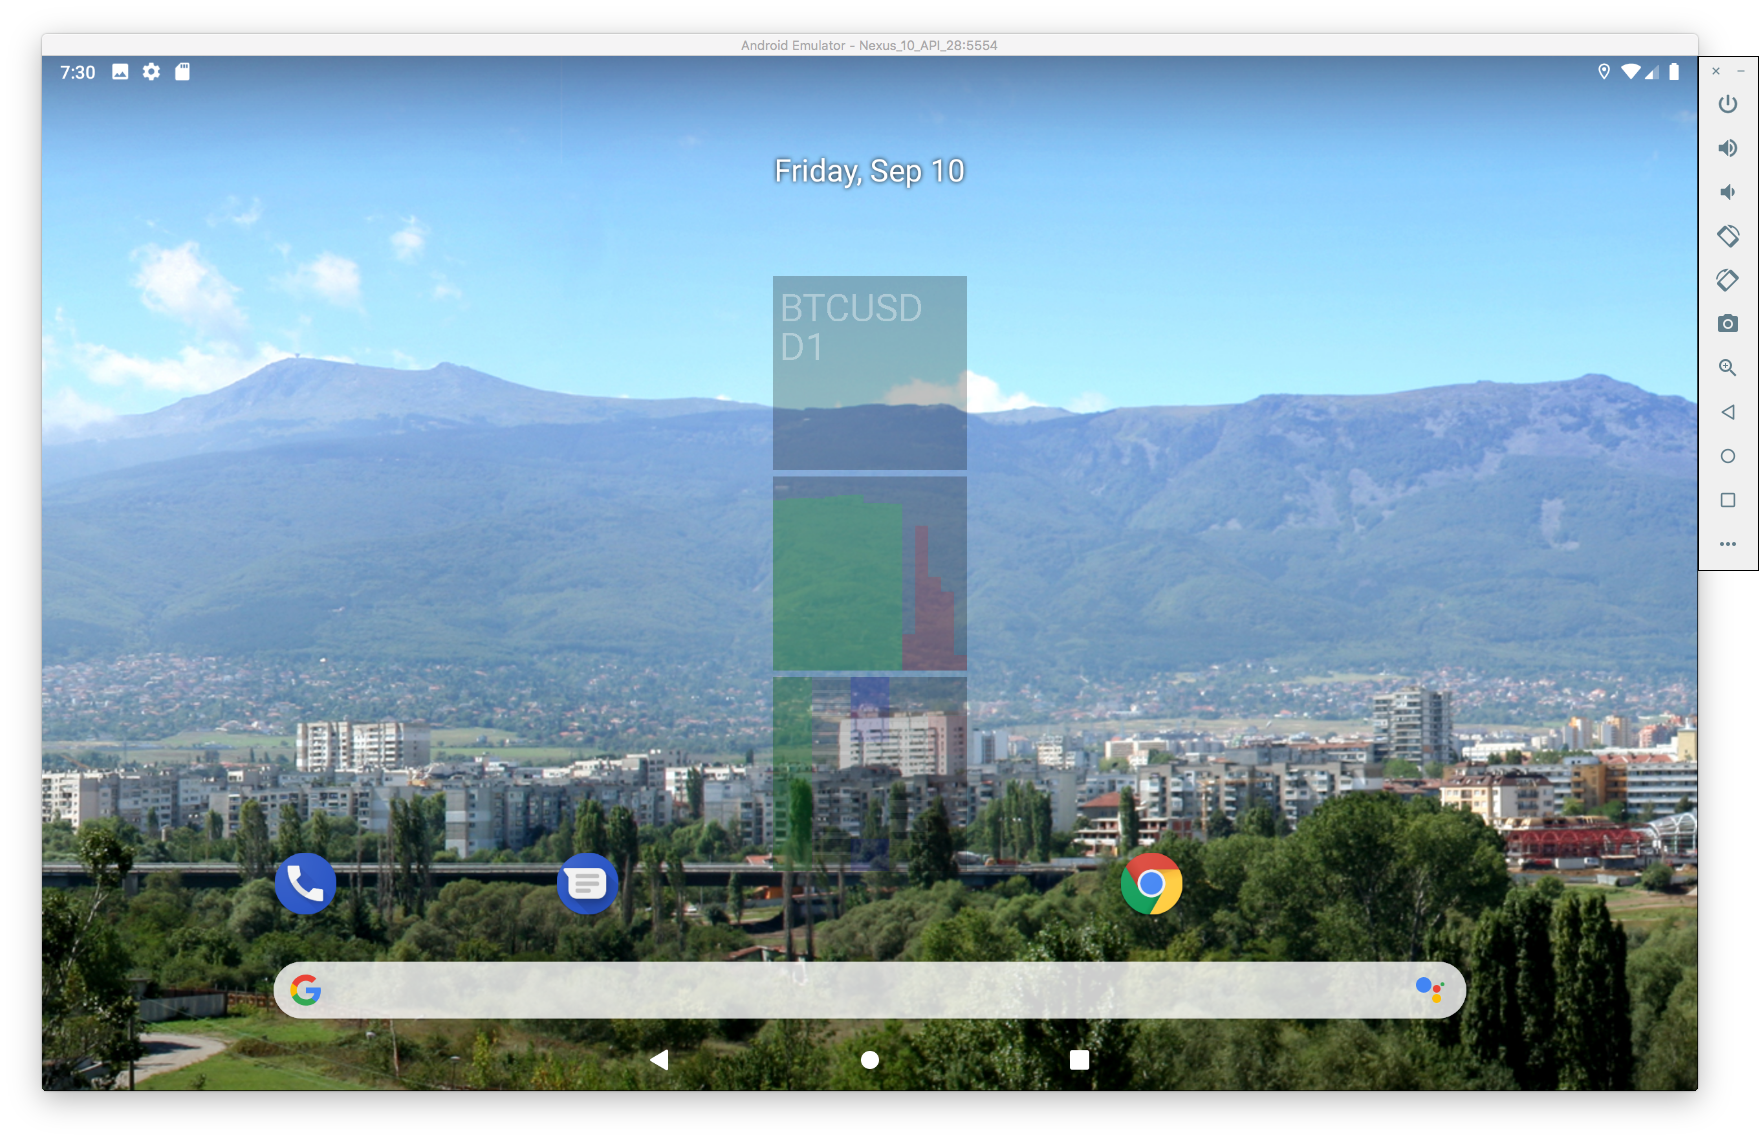
\includegraphics[width=1.0\linewidth]{fig01.png}}
\caption{Android Live Wallpaper distributed computing}
\label{fig01}
\end{figure}

The wallpaper has the following settings (Fig. \ref{fig02}) - the URL address of the remote server (Fig. \ref{fig03}), device loading (Fig. \ref{fig04}), positions of the panels (Fig. \ref{fig05}), and size of the panels (Fig. \ref{fig06}).

\begin{figure}[htbp]
\centerline{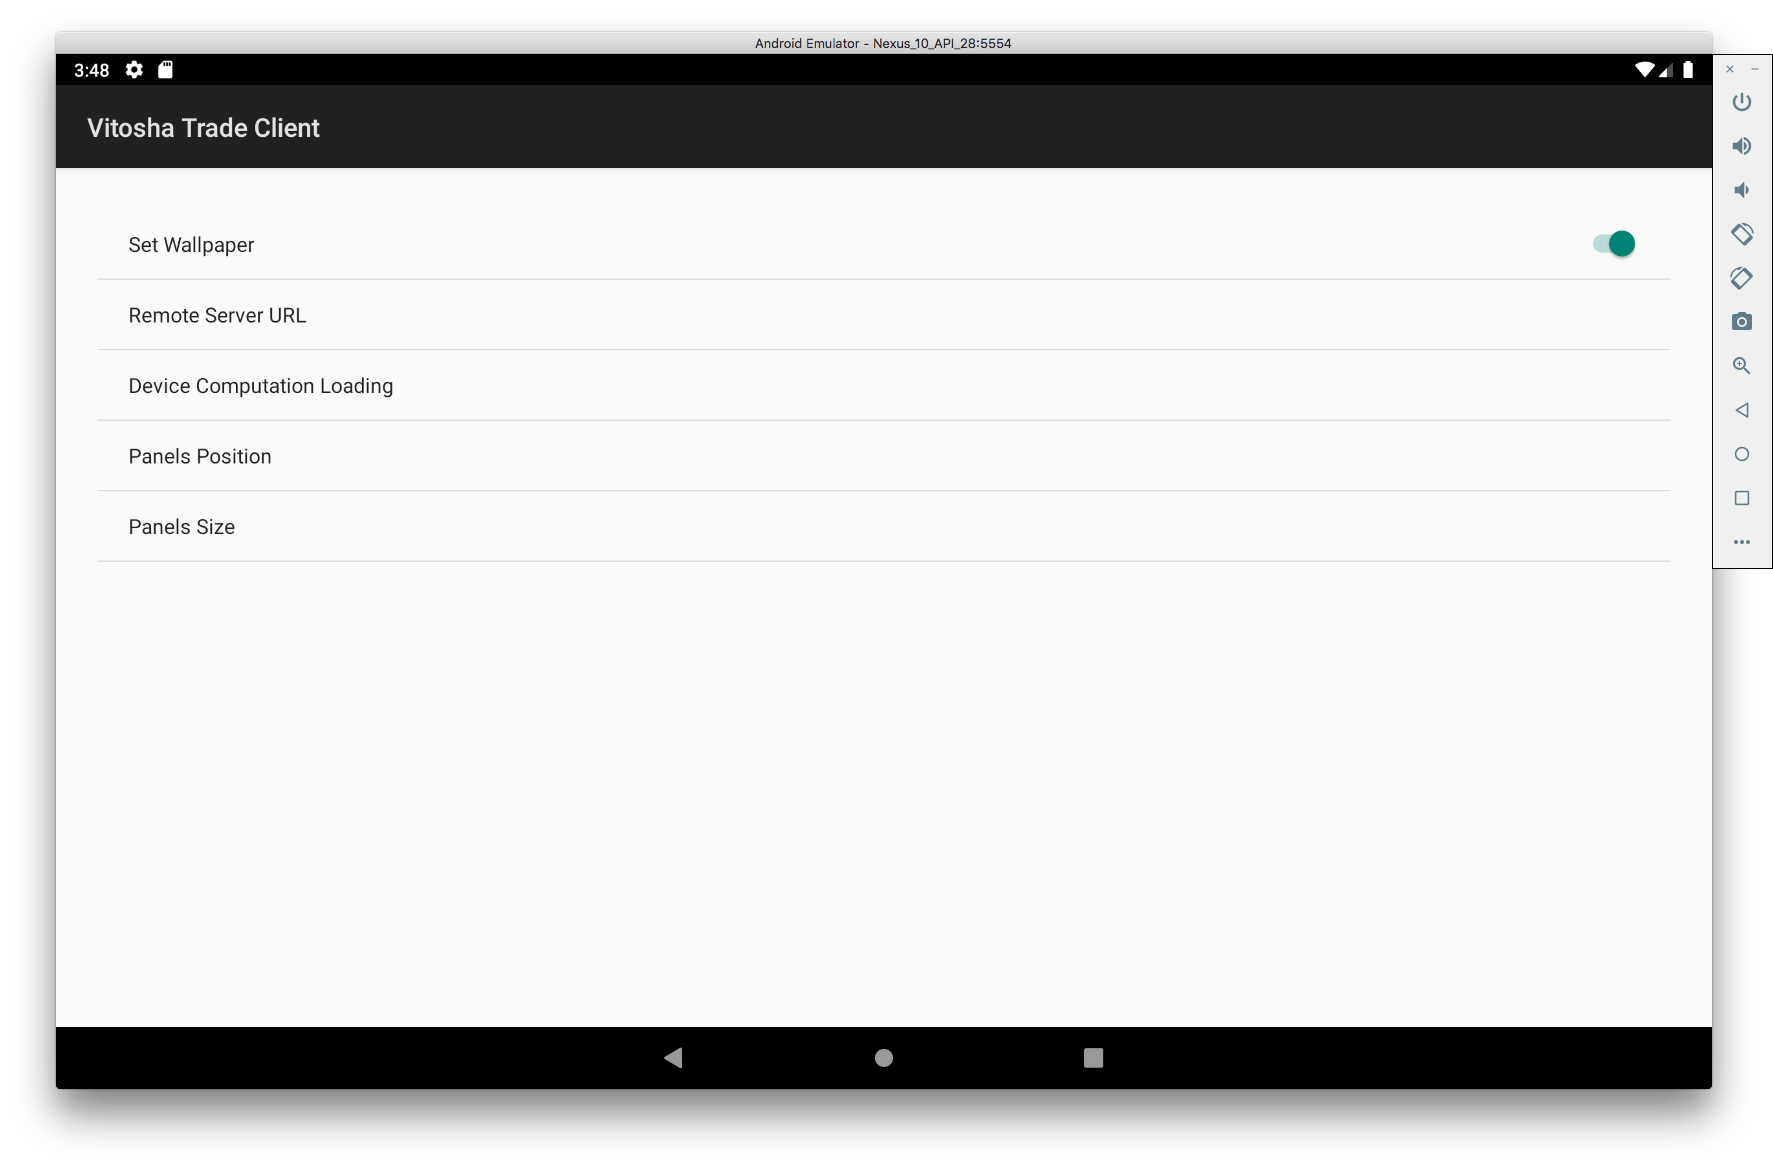
\includegraphics[width=1.0\linewidth]{fig02.png}}
\caption{Wallpaper performance settings}
\label{fig02}
\end{figure}

\begin{figure}[htbp]
\centerline{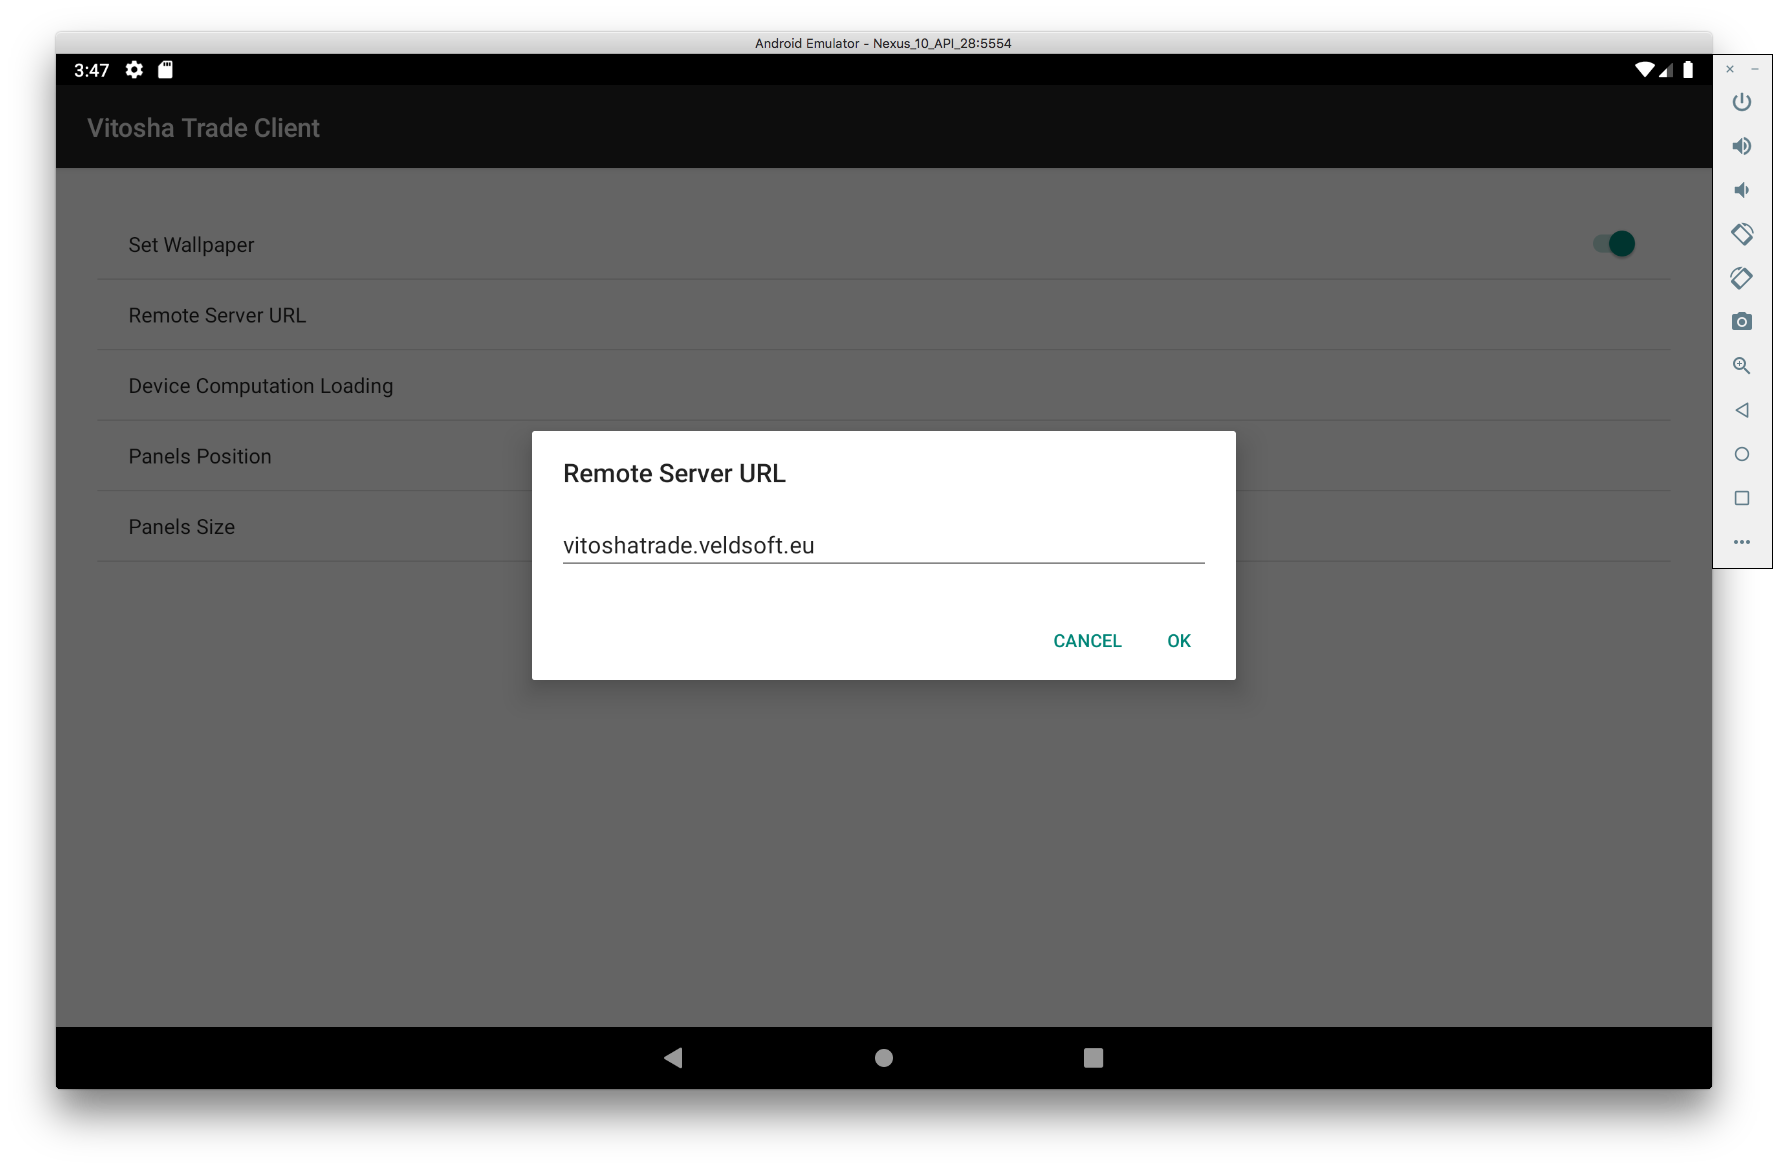
\includegraphics[width=1.0\linewidth]{fig03.png}}
\caption{Remote server URL address}
\label{fig03}
\end{figure}

\begin{figure}[htbp]
\centerline{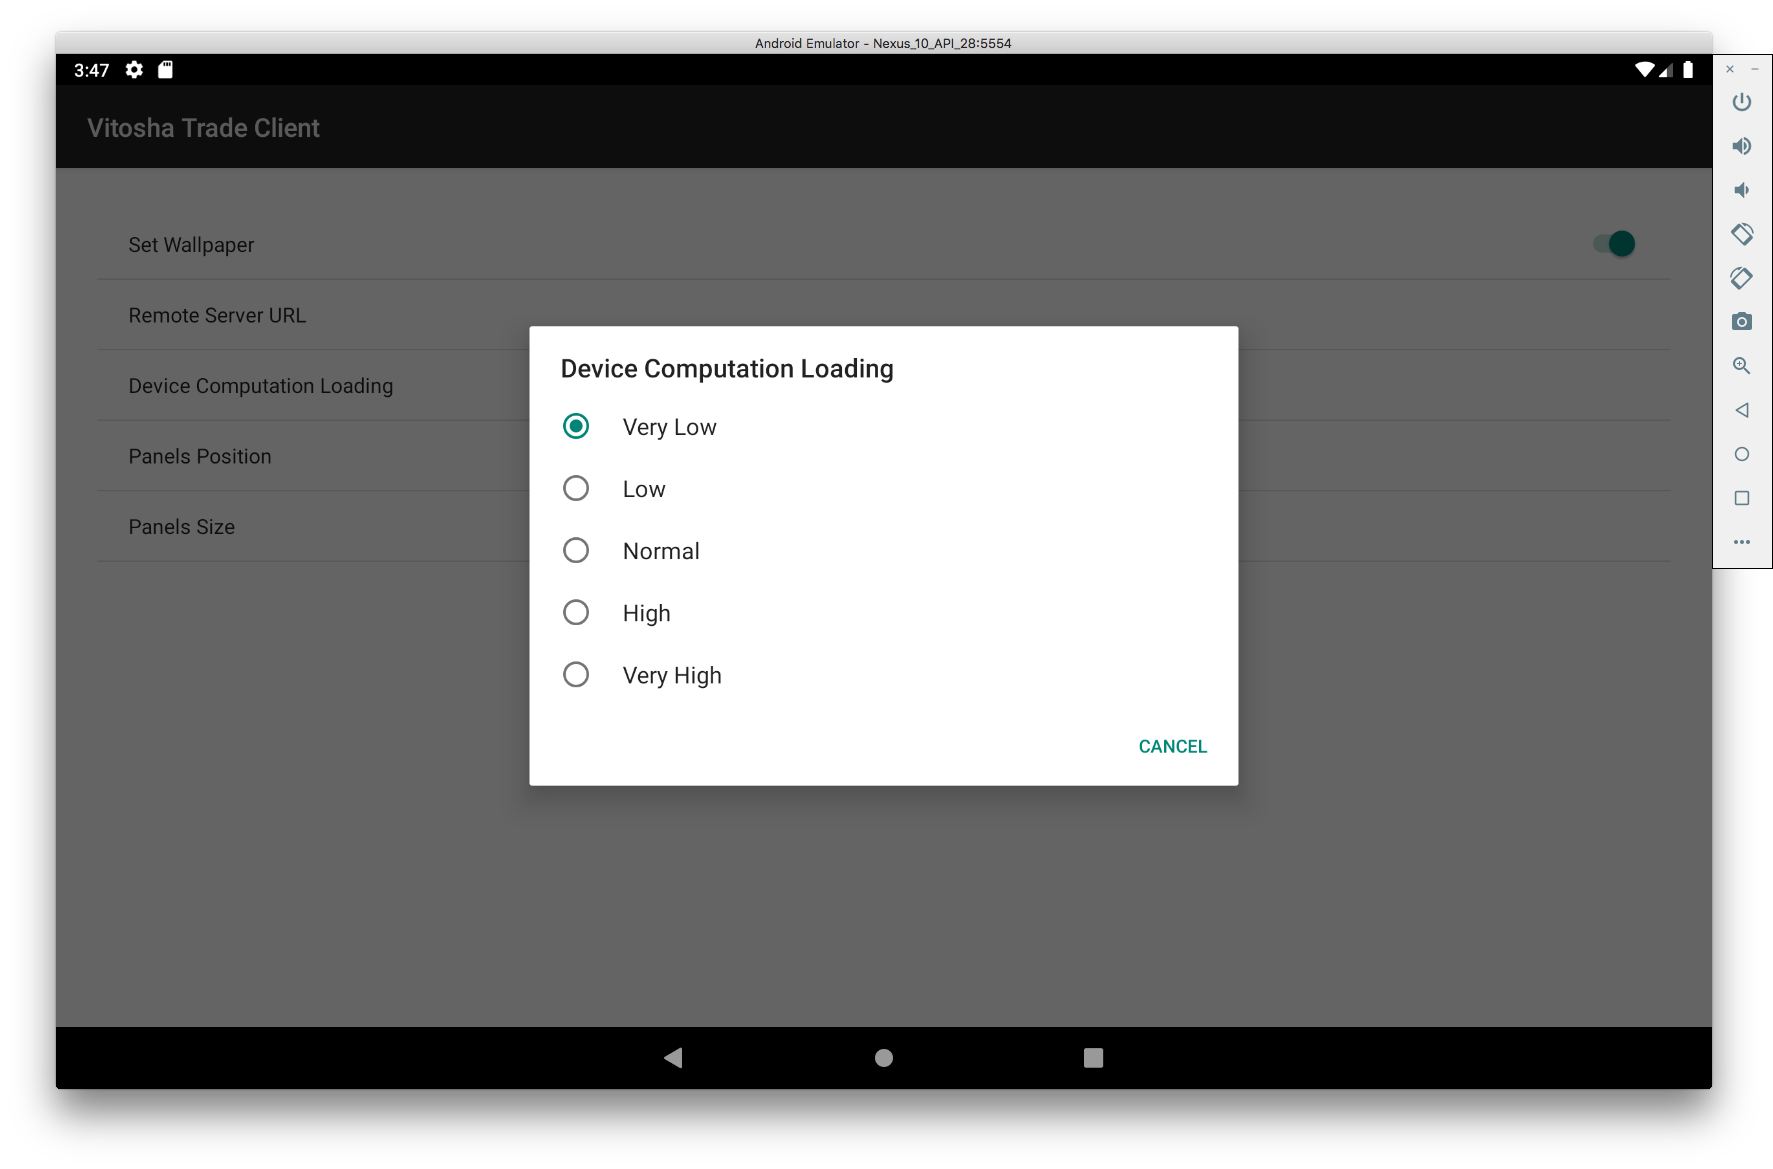
\includegraphics[width=1.0\linewidth]{fig04.png}}
\caption{Device background calculations loading}
\label{fig04}
\end{figure}

\begin{figure}[htbp]
\centerline{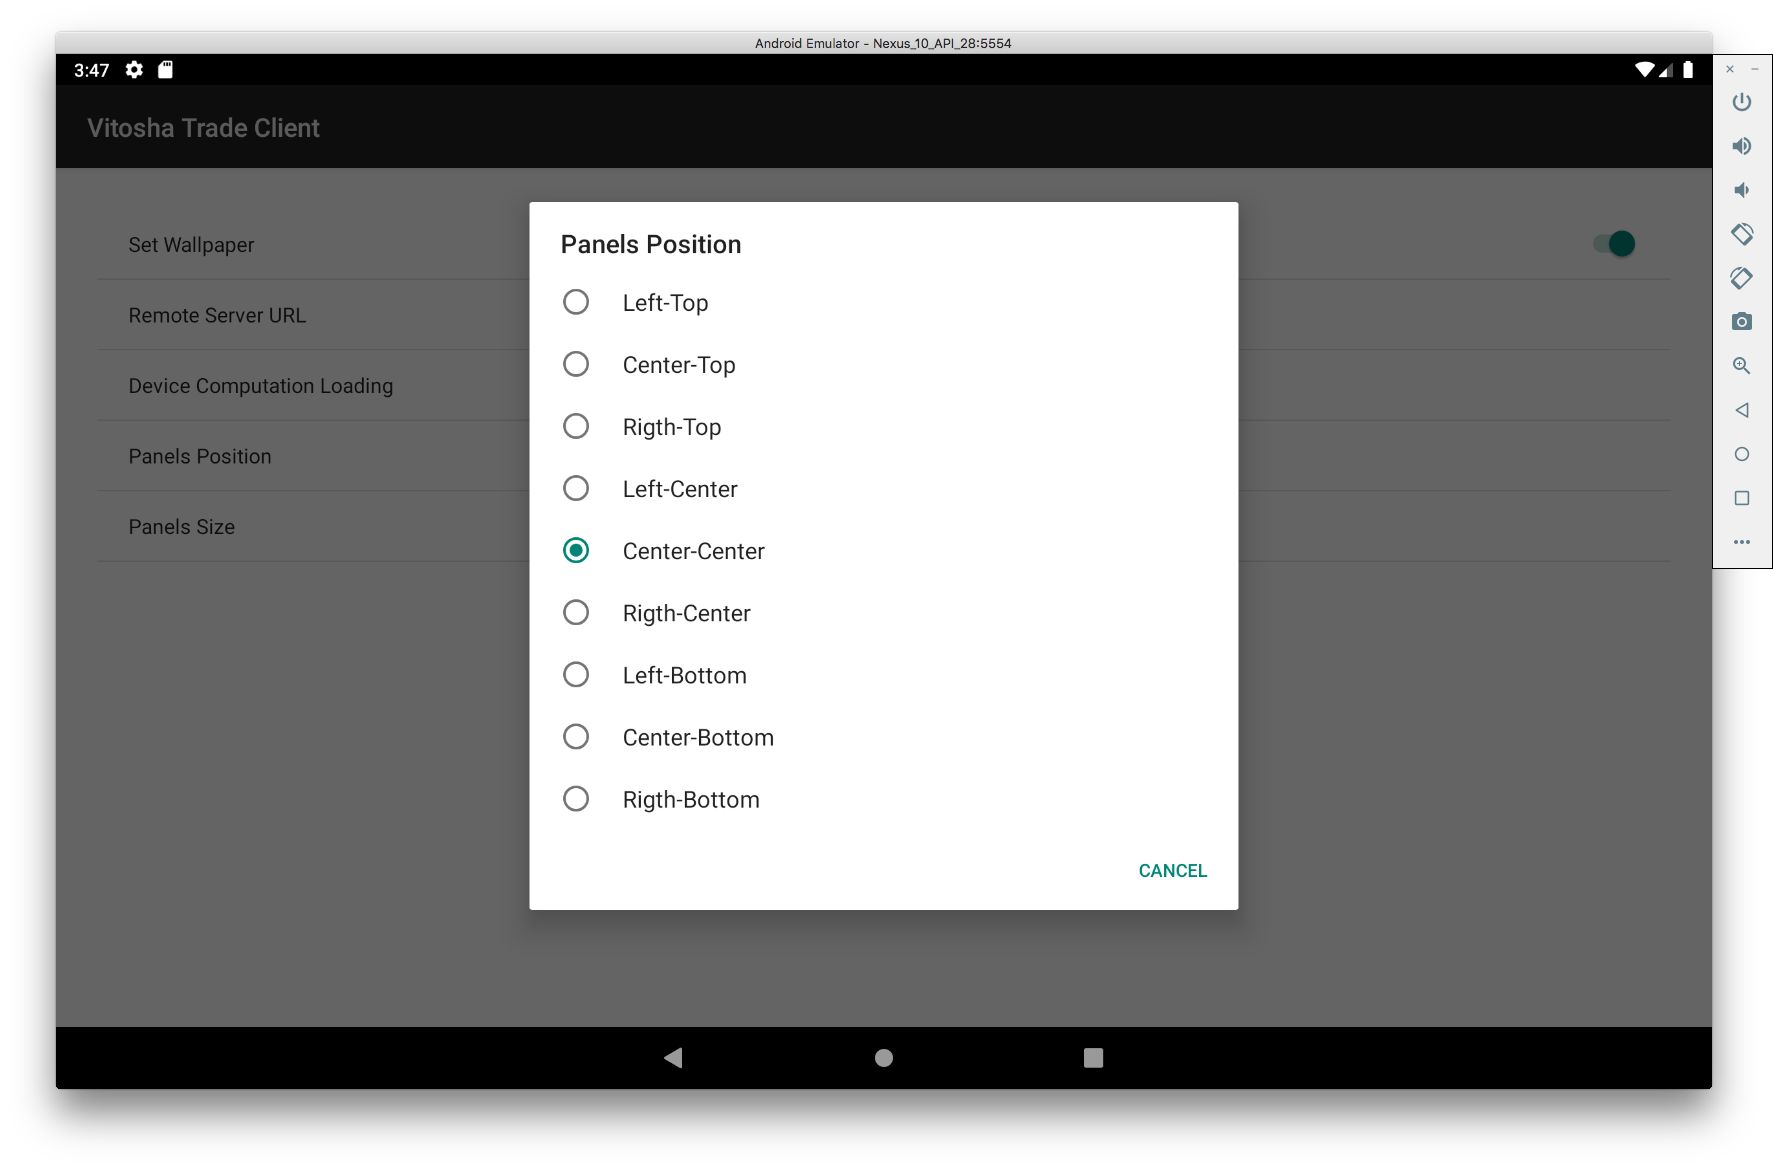
\includegraphics[width=1.0\linewidth]{fig05.png}}
\caption{Position of the panels}
\label{fig05}
\end{figure}

\begin{figure}[htbp]
\centerline{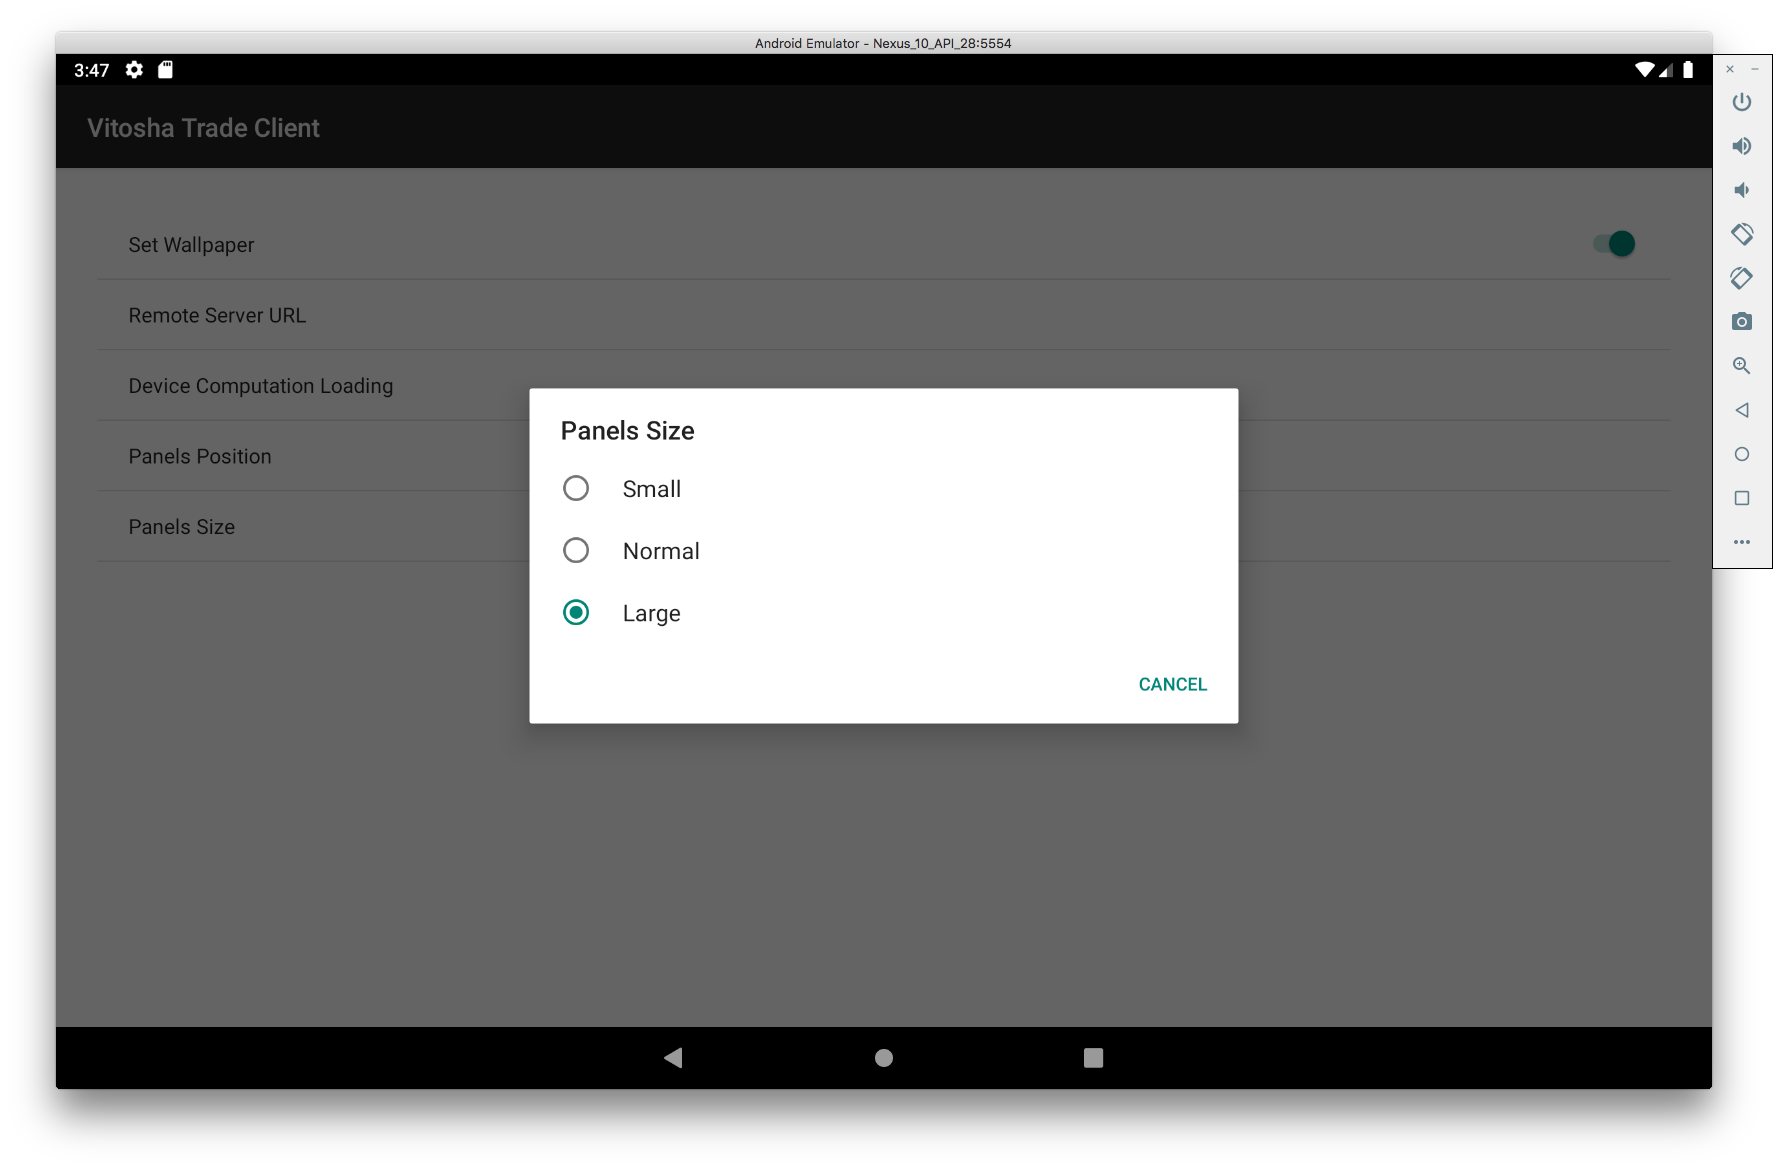
\includegraphics[width=1.0\linewidth]{fig06.png}}
\caption{Size of the panels}
\label{fig06}
\end{figure}

The mobile client application is written in such a way that the calculations can be performed even when the mobile device is offline on the Internet. This is achieved by storing the calculation information in a local copy of the SQLite relational database. If it is not possible to request a calculation package from the remote server, a package from the local database is loaded. 

\begin{figure}[htbp]
\centerline{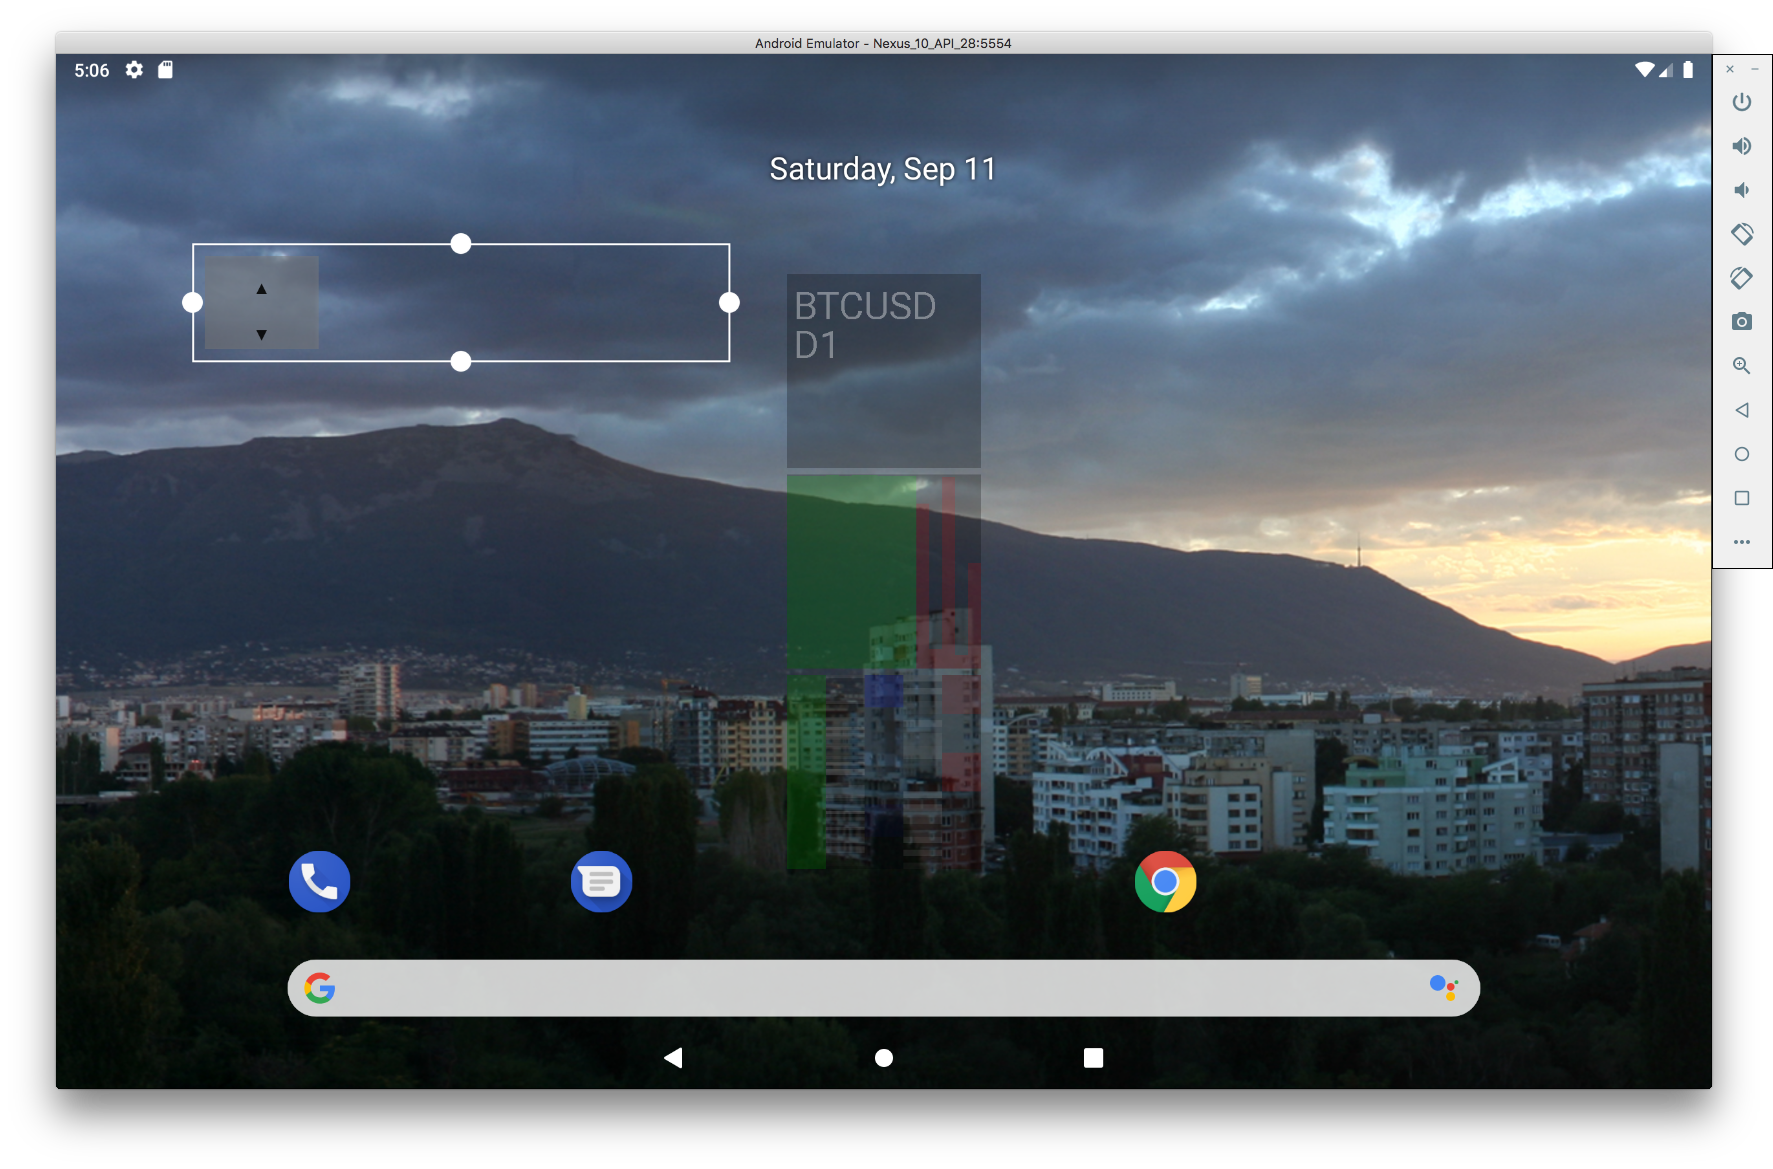
\includegraphics[width=1.0\linewidth]{fig07.png}}
\caption{A voting widget}
\label{fig07}
\end{figure}

\begin{figure}[htbp]
\centerline{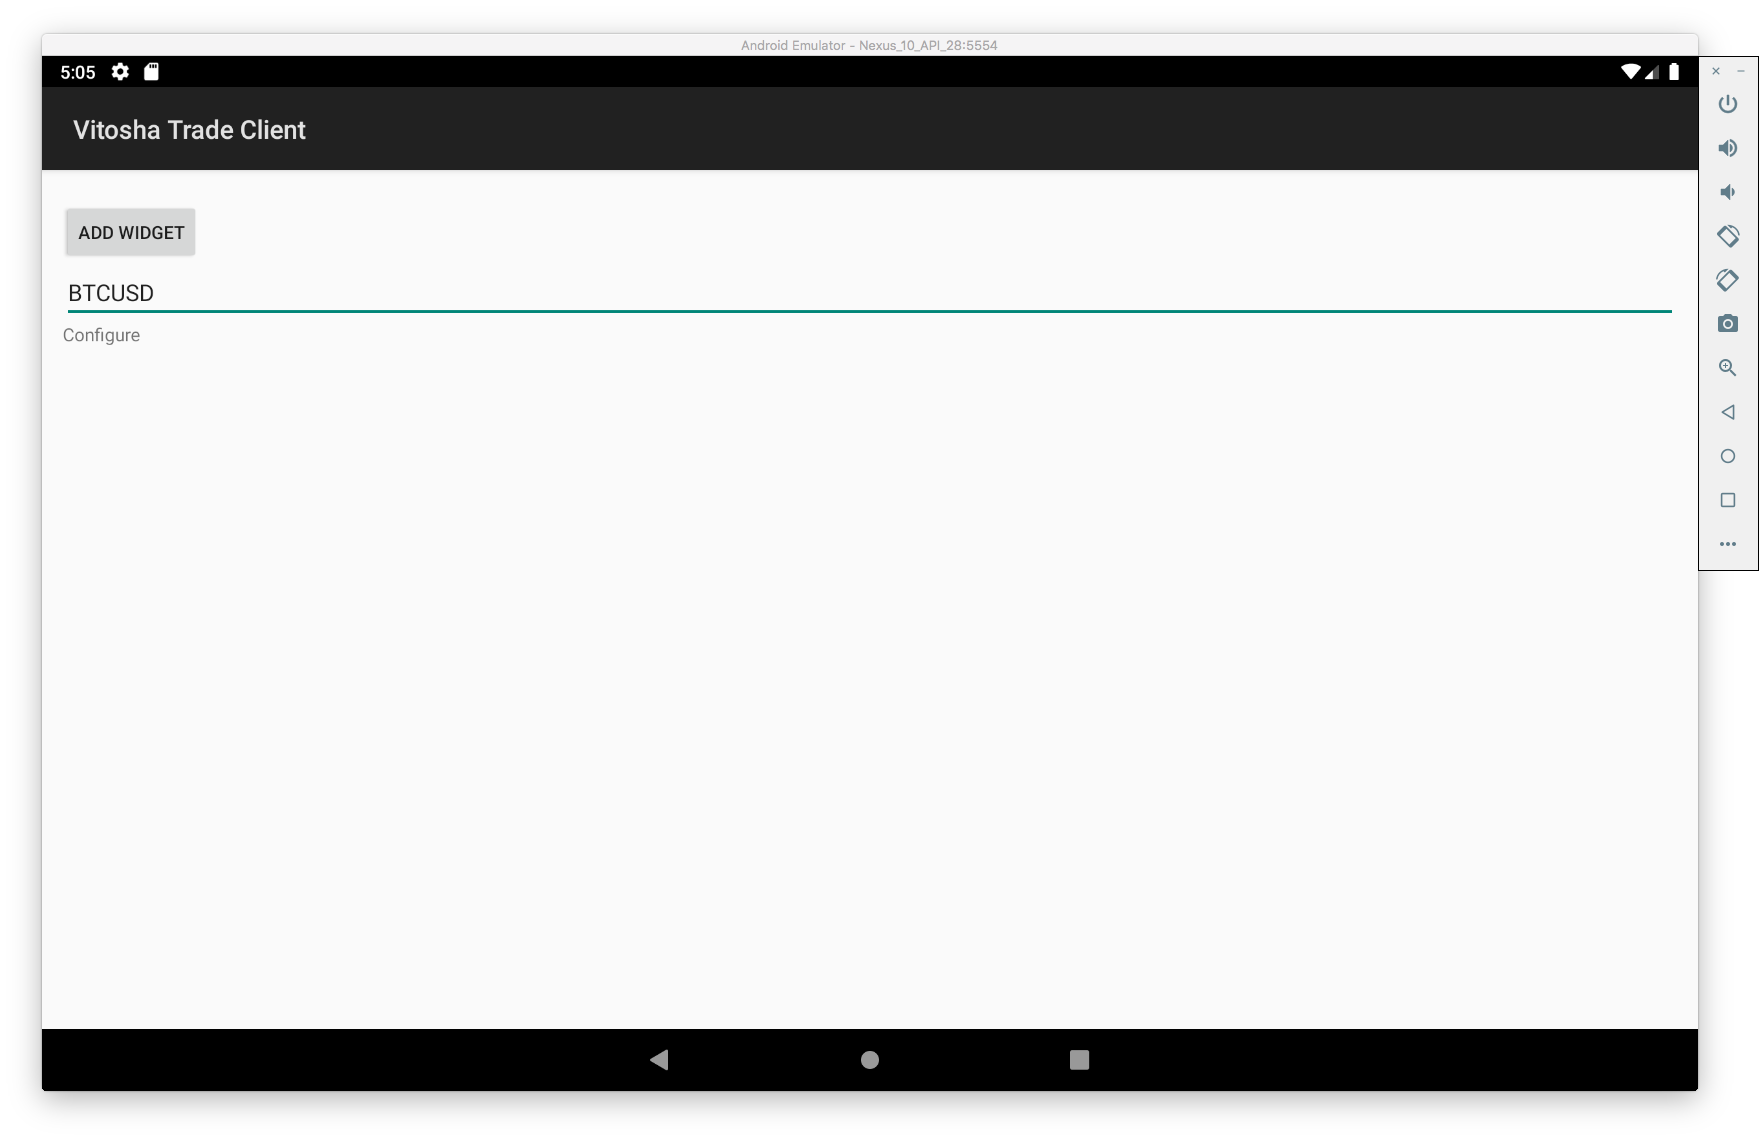
\includegraphics[width=1.0\linewidth]{fig08.png}}
\caption{Settings of the voting widget}
\label{fig08}
\end{figure}

In some projects for distributed computing, it is impossible to calculate the quality of the obtained solutions numerically. Examples of such projects are situations in which a subjective assessment of beauty is needed. Another situation is subjective human intuition. Many people make many decisions based on their intuitive opinion. It is popular to do stock exchange trading, done only because of the feeling that a certain company will perform well. Decisions made by people only through intuition are difficult to explain logically. The fact that decisions are difficult to explain does not mean that these decisions cannot be correct in most cases. The intuitive solution is the result of a large amount of information that people receive on a daily basis and is very often processed mainly on a subconscious level. Such information processing is not possible with modern computers. The information, processed in such a way, can be collected in human-computer distributed computing. In a financial forecasting system, the user can be asked to vote for prices up or down. Android Widgets are the perfect tool for gathering such voting information (Fig. \ref{fig07}). Widgets are not only static visualizers, but they can handle user input. The votes are first stored in the local SQLite database and then sent to the remote server. The important information is which financial instrument is being voted on, when the voting took place in time and what is the voting direction. The voting information is classified on the server-side according to the frequency of voting and the success of the voting assumption \cite{Ketipov-01}. The voting widget has a settings dialog itself (Fig. \ref{fig08}).

Because Android OS allows external libraries written in Java, it gives almost unlimited possibilities for machine learning. The modular development of the project allows calculations to be done even on desktop machines by recompilation of the client source code \cite{Balabanov-01}. Such organization of the source code allows mobile devices to work in parallel with desktop computers. Different metaheuristics can be involved in artificial neural networks training. By its communications and user interface capabilities, Android OS is a perfect candidate for distributed computing projects. The rapid development of mobile hardware will offer great computing power in the near future. 

\section{Conclusion}

This study presents the capabilities of the Android OS for the implementation of donated distributed computing. The capabilities of the operating system are demonstrated with an application for training artificial neural networks. The training has been done with population-based heuristics for global optimization. The artificial neural network has been trained to forecast time series. The efficiency of mobile distributed computing has been proven, but testing of the system is still in progress. 

Having all these distributed computing capabilities in Android OS is inspiring, but as further research, it will be interesting what can be done with iOS devices and Kai OS devices. 

\section*{Acknowledgment}

This research is funded by Velbazhd Software LLC and it is partially supported by the Bulgarian Ministry of Education and Science (contract D01–205/23.11.2018) under the National Scientific Program ``Information and Communication Technologies for a Single Digital Market in Science, Education and Security (ICTinSES)'', approved by DCM \# 577/17.08.2018.

\begin{thebibliography}{00}

\bibitem{Apache-01} Apache HttpClient from Android, The Apache Software Foundation, 2021. https://hc.apache.org/httpcomponents-client-4.5.x/android.html

\bibitem{Balabanov-01} T. Balabanov, Vitosha Trade Android Client, Velbazhd Software LLC, 2021. https://github.com/TodorBalabanov/Vitosha-Trade-Android-Client

\bibitem{Chinara-01} S. Chinara, S. Rath, Energy Efficient Mobility Adaptive Distributed Clustering Algorithm for Mobile Ad Hoc Network, Proceedings of International Conference on Advanced Computing and Communications, pp. 265-272, 2008.

\bibitem{Durrani-01} M. Durrani, A. Shamsi, Volunteer computing: requirements, challenges, and solutions, Journal of Network and Computer Applications, vol. 39, pp. 369-380, 2014.

\bibitem{Forcier-01} K. Forcier, Never Idle: The Animated Screensaver and the Culture of Always-On Computing, Afterimage, vol. 48, no. 2, pp. 79–93, 2021.

\bibitem{Geng-01} J. Geng, D. Li, Y. Cheng, S. Wang, J. Li., HiPS: Hierarchical Parameter Synchronization in Large-Scale Distributed Machine Learning, Proceedings of the 2018 Workshop on Network Meets AI \& ML, Association for Computing Machinery, New York, NY, USA, pp. 1-7,  2018.

\bibitem{Google-01} Google Developers, Services Overview, Google LLC, 2021. https://developer.android.com/guide/components/services

\bibitem{Google-02} Google Developers, App Widgets Overview, Google LLC, 2021. https://developer.android.com/guide/topics/appwidgets/overview

\bibitem{Grouchnikov-01} K. Grouchnikov, Live wallpapers with Android SDK 2.1, Pushing Pixels, 2010. https://www.pushing-pixels.org/2010/02/01/live-wallpapers-with-android-sdk-2-1.html

\bibitem{Guler-01} H. Guler, B. Cambazoglu, O. Ozkasap, Task allocation in volunteer computing networks under monetary budget constraints, Peer-to-Peer Networking and Applications, vol. 8, pp. 938-951, 2015.

\bibitem{Hadka-01} D. Hadka, MOEA Framework, A Free and Open Source Java Framework for Multiobjective Optimization, http://moeaframework.org/

\bibitem{Heaton-01} J. Heaton, Encog Machine Learning Framework, Heaton Research Inc., 2020. https://www.heatonresearch.com/encog/

\bibitem{Heien-01} E. Heien, D. Anderson, K. Hagihara, Computing Low Latency Batches with Unreliable Workers in Volunteer Computing Environments, Journal of Grid Computing, vol. 7, pp. 501, 2009.

\bibitem{Ketipov-01} R. Ketipov, G. Kostadinov, P. Petrov, I. Zankinski, T. Balabanov, Human-Computer Mobile Distributed Computing for Time Series Forecasting, Proceedings of Distributed Computer and Communication Networks, Communications in Computer and Information Science, Springer, Cham, vol. 1141, pp. 503-509, 2019.

\bibitem{Krieger-01} E. Krieger, G. Vriend, Models@Home: distributed computing in bioinformatics using a screensaver based approach, Bioinformatics, vol. 18, no. 2, pp. 315-318, 2002.

\bibitem{Lamport-01} L. Lamport, N. Lynch, Distributed Computing: Models and Methods, Handbook of Theoretical Computer Science, Formal Models and Semantics, pp. 1157-1199, 1990.

\bibitem{Leary-01} S. Leary, JSON in Java [package org.json], 2021. https://github.com/stleary/JSON-java

\bibitem{Meyerov-01} I. Meyerov, S. Bastrakov, A. Sysoyev, V. Gergel, Comprehensive Collection of Time-Consuming Problems for Intensive Training on High Performance Computing, Communications in Computer and Information Science, vol. 965, Springer, Cham, pp. 523-530, 2019.

\bibitem{Pfahnl-01} A. Pfahnl, Properties of fast-decay cathode-ray tube phosphors, The Bell System Technical Journal, vol. 42, no. 1, pp. 181-201, 1963.

\bibitem{Sebera-01} M. Sebera, HttpClient Android Library, 2019. https://github.com/smarek/httpclient-android

\bibitem{Tapparello-01} C. Tapparello, C. Funai, S. Hijazi, A. Aquino, B. Karaoglu, H. Ba, J. Shi, W. Heinzelman, Volunteer Computing on Mobile Devices: State of the Art and Future Research Directions, Mobile Computing and Wireless Networks: Concepts, Methodologies, Tools, and Applications, pp. 2171-2198, 2016.

\bibitem{Vogel-01} L. Vogel, Android Live Wallpaper - Tutorial, Vogella GmbH, 2020. https://www.vogella.com/tutorials/AndroidLiveWallpaper/article.html

\end{thebibliography}

\end{document}
